\subsection{Restructuring}
After transitioning from cold geometry to hot geometry and accounting for thermal expansion, the fuel restructuring process must be considered. This involves assumptions about the radii of columnar and equiaxed regions as well as the corresponding densities in these regions. According to Holander’s book, the temperature boundaries are set at 1800°C for the columnar region and 1600°C for the equiaxed region. Regarding densities, the as-fabricated region retains its original density, while the equiaxed region is assumed to have 95\% of the theoretical density (TD) and the columnar region 98\% of TD.

Initially, the columnar and equiaxed radii are evaluated at 1800°C and 1600°C, respectively, based on a temperature map. This map provides temperature values at various heights along the fuel pin and utilizes a precise function to determine the temperature at any position within the previously developed 3D model.

Once the columnar and equiaxed radii are determined, the void radius is calculated. The as-fabricated region corresponds to the remaining portion of the fuel outer radius after subtracting the equiaxed region. The following equation is used to estimate the void formation radius:
\begin{equation}
R_{\text{void}} = \sqrt{
    R_{\text{col}}^2 - R_{\text{eq}}^2 \cdot \left( \frac{\text{Density}_{\text{AS}}}{\text{Density}_{\text{col}}} \right)
    + \left( R_{\text{eq}}^2 - R_{\text{col}}^2 \right) \cdot \left( \frac{\text{Density}_{\text{eq}}}{\text{Density}_{\text{AS}}} \right)
}
\end{equation}

Finally, the relationship between height and radius is plotted to illustrate the restructuring phenomenon and highlight the axial position dependence (z-axis) of the fuel pin. Figure~\ref{fig:restructuring} shows the restructuring effect, with a particular focus on cladding swelling due to void formation.

\begin{figure}[H]
\centering
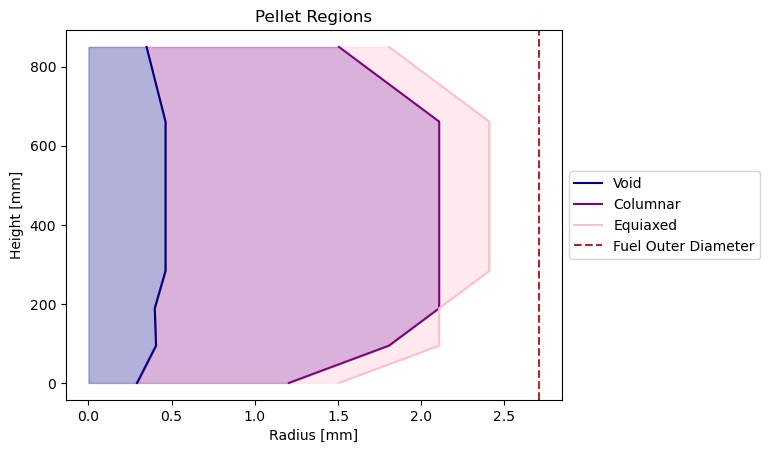
\includegraphics[width=0.8\textwidth]{restructuring.png}
\caption{Cladding swelling due to void formation.}
\label{fig:restructuring}
\end{figure}
